\documentclass[a4paper,oneside,12pt,notitlepage]{article}

\usepackage[utf8]{inputenc}
\usepackage[portuges]{babel}
\usepackage{graphics}
\usepackage{palatino}
\usepackage{geometry}

\geometry{paperwidth=210mm,paperheight=297mm,
          textwidth=150mm,textheight=210mm,
          top=30mm,bottom=30mm,
          left=30mm,right=30mm}

\frenchspacing
\linespread{1.3}

\title{Lamentos de um Matemático}
\author{Paul Lockhart}
\date{}

\begin{document}

\maketitle

Um músico acorda de um terrível pesadelo.
Em seu sonho ele se encontra numa sociedade onde a educação musical tornou-se obrigatória.
``Nós estamos ajudando nossos estudantes a se tornarem mais competitivos num mundo cada vez mais cheio de sons''.
Educadores, sistemas de ensino e o Estado são os responsáveis por esse importante projeto.
Estudos foram feitos, comitês foram formados e decisões foram feitas -- tudo sem a participação de um músico ou compositor.

Como músicos são conhecidos por registrarem suas ideias em forma de partituras, esses curiosos pontos e linhas pretas devem constituir a ``linguagem da música''.
É imperativo que os estudantes tornem-se fluentes nessa linguagem se eles almejam atingir qualquer grau de competência musical;
de fato, seria ridículo esperar que uma criança cantasse ou tocasse um instrumento sem ter uma boa base de notação e teoria musical.
Tocar e escutar música ou ficar sozinho compondo uma peça original são considerados tópicos muito avançados, por isso são geralmente adiados ao menos para a graduação e mais frequentemente para a pós-graduação.

No Ensino Fundamental o objetivo é treinar os estudantes no uso dessa linguagem -- manipular símbolos de acordo com um conjunto fixo de regras:
``Aula de música é onde nós pegamos nosso caderno pautado, nosso professor coloca algumas notas no quadro e nós copiamos ou transpomos elas para um tom diferente.
Nós não podemos errar ao copiar as claves e as armaduras e nosso professor é muito exigente sobre pintar as semínimas completamente.
Uma vez tivemos um problema de escala cromática e eu acertei, mas o professor não me deu crédito porque eu coloquei as hastes no lado errado''.

No auge de sua sabedoria, os educadores logo perceberam que mesmo crianças muito novas podem receber este tipo de instrução musical.
De fato é considerado vergonhoso um garoto de terceira série não ter memorizado completamente o ciclo de quintas.
``Eu vou ter que levar meu filho a um professor particular.
Ele não se dedica aos seus deveres de música.
Diz que é chato.
Apenas senta lá, olha pela janela, cantarola para si mesmo e faz músicas bobas''.

Nas séries mais avançadas a pressão é mais forte.
Afinal, os estudantes precisam ser preparados para as tradicionais provas e para o vestibular.
Estudantes precisam ter aula de Escalas e Modos, Métrica, Harmonia e Contraponto.
``É bastante coisa pra aprender, mas depois na faculdade quando eles finalmente ouvirem tudo isso eles vão realmente apreciar o trabalho que fizeram no Ensino Médio''.
É claro que não são muitos estudantes que vão se dedicar à música, então apenas alguns irão escutar os sons que os pontos pretos representam.
De qualquer forma, é muito importante que todo membro da sociedade possa reconhecer uma modulação ou uma passagem fugal, não importa que eles nunca ouçam uma.
``Para dizer a verdade, a maioria dos estudantes não é muito boa em música.
Eles ficam entediados na sala, não tem habilidade e suas tarefas de casa são quase ilegíveis.
A maioria deles não se importa em como a música é importante no mundo de hoje;
eles apenas querem fazer o menor número possível de cursos de música pra terminar de uma vez.
Eu acho que existem pessoas que nasceram pra música e outras que não.
Eu tive uma criança que, cara, era sensacional!
Suas partituras eram impecáveis -- cada nota no lugar certo, caligrafia perfeita, sustenidos, bemóis, simplesmente lindos.
Ela será uma tremenda musicista um dia.''

Ao acordar suando frio o músico se dá conta que, felizmente, foi tudo apenas um sonho maluco.
``É claro!'' ele diz a si mesmo,
``Nenhuma sociedade reduziria uma forma de arte tão bonita e significativa para algo tão estúpido e trivial;
nenhuma cultura seria tão cruel com suas crianças a ponto de privá-las de uma expressão humana tão natural.
Que absurdo!''

Enquanto isso, do outro lado da cidade, um pintor acabara de acordar de um pesadelo semelhante\ldots

\vspace{1em}

Eu me surpreendi ao me ver numa sala de aula convencional -- sem cavaletes, sem tubos de tinta.
``Ah, nós não pintamos antes do Ensino Médio'',
me disseram os estudantes.
``Passamos a sétima série estudando cores e aplicadores''.
Eles me mostraram uma planilha.
De um lado estavam amostras de cores separadas por espaços em branco.
Eles deveriam escrever seus nomes.
``Eu gosto de pintura'',
um deles fez questão de dizer,
``me dizem o que fazer e eu faço. É fácil!''

Após a aula eu fui falar com o professor.
``Então seus estudantes não fazem nenhuma pintura?''
perguntei.
``Bem, no próximo ano eles terão Pré-Pintura-por-Números.
% Há algum termo melhor pra Paint-by-Numbers?
Isso prepara eles para o Pintura-por-Números que terão no Ensino Médio.
Então eles poderão usar o que aprenderam aqui e aplicar em situações de pintura da vida-real -- mergulhando o pincel na tinta, limpando-o, coisas assim.
É claro que nós selecionamos nossos estudantes por habilidade.
Os que são realmente excelente pintores -- aqueles que sabem suas cores e pincéis até de trás pra frente -- podem pintar um pouco mais cedo e algum deles até assistem aulas de Localização Avançada por créditos de faculdade.
% Essa frase ficou estranha e deve haver uma tradução melhor que Localização Avançada. Quem puder, modifique.
% Não seriam aulas para o exame de "placement", ou seja, para validar alguma "disciplina"?
% De fato faz bem sentido que localização... Então seria algo como: "até assistem aulas que depois podem validar na universidade"? Quem quiser pode mudar.
Porém, nós estamos apenas tentando dar a essas crianças uma boa base de o que é pintura, então quando eles saírem daqui para o mundo real e forem pintar sua cozinha eles não façam uma bagunça nela''.

``Hmmm, essas aulas no Ensino Médio que você mencionou\ldots{}''

``Pintura-por-números?
Nós estamos tendo muitas inscrições ultimamente.
Acho que a maioria vem por causa dos pais que querem garantir que suas crianças entrem em boas faculdades.
Nada parece melhor que Pintura-por-números Avançada num histórico de Ensino Médio''.
% Pode ser conveniente colocar uma nota de rodapé explicando como é a educação nos Estados Unidos.

``Por que as faculdades se importam com você conseguir preencher regiões numeradas com as cores correspondentes?''

``Ah, bem, você sabe, isso mostra um lúcido raciocínio lógico.
E é claro que se um estudante está planejando se formar numa ciência visual, como moda ou design de interiores, então é realmente uma boa ideia já sair do Ensino Médio com seus pré-requisitos relacionados a pintura''.

``Entendo.
E quando os estudantes podem pintar livres, numa folha em branco?''

``Você parece um de meus professores!
Eles sempre vem com essa de expressar os sentimentos e coisas desse tipo -- coisas abstratas que não tem realmente nada a ver.
% As novas normas do português eliminaram o acento de têm :)
Eu sou formado em Pintura e nunca trabalhei muito numa folha em branco.
Eu apenas uso os kits Paint-by-Numbers distribuídos pelo conselho escolar''.
% Convém revisar toda essa parte de pintura, não ficou muito boa.

\vspace{1em}

\begin{center}
***
\end{center}

\vspace{1em}

Infelizmente, nosso atual sistema de ensino de matemática é precisamente este tipo de pesadelo.
De fato, se eu tivesse que projetar um mecanismo com o propósito explícito de \textsl{destruir} a curiosidade natural de uma criança e seu prazer em criar padrões, não conseguiria fazer melhor do que está sendo feito atualmente -- eu simplesmente não teria a criatividade necessária para inventar ideias sem sentido e dolorosas como as que constituem o ensino de matemática contemporâneo.

Todos sabem que algo está errado.
Os políticos dizem, ``precisamos de padrões mais altos''.
As escolas dizem, ``precisamos de mais dinheiro e equipamentos''.
Educadores dizem uma coisa e professores dizem outra.
Estão todos errados.
As únicas pessoas que entendem o que está acontecendo são as que mais levam a culpa e são menos ouvidas: os alunos.
Eles dizem ``a aula de matemática é estúpida e entediante'' e tem razão.
% Mudei de "inútil" pra "estúpida" porque acho que é mais o que o Paul quis dizer, mas se alguém encontrar adjetivos melhores pode mudar. A frase original é: "math class is stupid and boring"

\section*{Matemática e Cultura}

A primeira coisa a entender é que matemática é uma arte.
A diferença entre matemática e as outras artes, tais como música e pintura, é que nossa cultura não a reconhece como tal.
Todos entendem que poetas, pintores e músicos criam obras de arte e se expressam por palavras, imagens e sons.
De fato, nossa sociedade é bastante generosa quando se trata de expressão da criatividade: arquitetos, chefs e até diretores de televisão são considerados artistas profissionais. % alguma sugestão melhor que "artistas profissionais"?
Porque não matemáticos?

Parte do problema é que ninguém faz a mínima ideia do quê matemáticos fazem.
O senso comum parece ser que matemáticos estão de alguma forma ligados à ciência -- talvez eles ajudem cientistas com suas fórmulas, ou digitem números enormes em computadores por uma razão ou outra.
Não há dúvida que se se o mundo tivesse que ser dividido em os ``sonhadores poéticos'' e os ``pensadores racionais'', a maioria das pessoas classificaria os matemáticos na segunda categoria.

No entanto, o fato é que não há nada tão sonhador e poético, nada tão radical, subversivo e psicodélico quanto matemática.
Ela é precisamente tão instigante quanto cosmologia ou física (matemáticos \textsl{pensaram} em buracos negros muito antes que os astrônomos encontrassem algum) e dá mais liberdade de expressão que poesia, arte ou música (que dependem fortemente de propriedades do universo físico).
A matemática é a mais pura das artes e também a menos compreendida.

Então permitam-me tentar explicar o que é matemática e o que os matemáticos fazem.
Provavelmente a melhor maneira é começar com a excelente descrição de G. H. Hardy:

\begin{quote}
Um matemático, como um pintor ou poeta, é um criador de padrões.
Se seus padrões são mais permanentes que os deles, é porque são feitos com \textsl{ideias}.
\end{quote}

Então matemáticos ficam fazendo padrões de ideias.
Que tipo de padrões? Que tipo de ideias?
Ideias sobre rinocerontes? Não, essas deixamos para os biólogos.
Ideias sobre linguagem e cultura? Não, normalmente não.
Essas coisas são complicadas demais para o gosto dos matemáticos em geral.
Se existe algo como um conceito estético comum na matemática, é este: \textsl{o simples é belo}.
Matemáticos gostam de pensar sobre coisas as mais simples possíveis, e as coisas mais simples são \textsl{imaginárias}.

Por exemplo, se eu estou afim de pensar sobre formas -- e eu normalmente estou -- posso pensar em um triângulo dentro de uma caixa retangular:

\begin{center}
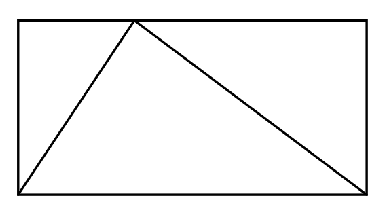
\includegraphics{triangle0.eps}
\end{center}

Eu imagino quanto da caixa o triângulo ocupa.
Dois terços, talvez?
O importante é entender que não estou falando desse \textsl{desenho} de um triângulo em uma caixa.
Nem estou falando de um objeto triangular de metal que forma as vigas de uma ponte. % alguma tradução melhor para "forming part of a girder system for a bridge"?
Não há nenhum outro propósito aqui.
Estou só \textsl{brincando}.
Isso é que é matemática -- pensar, brincar, entreter-se com sua imaginação.
A própria questão de quanto da caixa o triângulo ocupa nem faz \textsl{sentido} para objetos reais, físicos.
Até o triângulo físico feito com a maior precisão é ainda uma complicada coleção de átomos chacoalhantes; ele muda seu tamanho de uma hora para outra.
Isto é, a não ser que se queira falar sobre algum tipo de medida \textsl{aproximada}.
Bem, é aí que entra a estética.
Isto não é uma coisa simples, consequentemente é uma questão que depende de toda sorte de detalhes do mundo real.
Deixemos isso para os cientistas.
A questão \textsl{matemática} é sobre um triângulo imaginário dentro de uma caixa imaginária.
As extremidades são perfeita porque eu quero que elas sejam -- esse é o tipo de objeto sobre o qual prefiro pensar.
Este é um tema corrente em matemática: as coisas são o que você quer que sejam.
Você tem infinitas opções; a realidade não é um obstáculo.

Pelo outro lado, uma vez que tenha feito suas escolhas (por exemplo, eu posso escolher que meu triângulo seja simétrico, ou não), suas criaçõs fazem o que fazem, quer você goste, quer não.
Isto é o fascinante sobre fazer padrões imaginários: eles respondem!
O triângulo ocupa uma certa parte de sua caixa e eu não tenho controle sobre o quanto ocupa.
Existe um número, talvez seja dois terços, talvez não, mas eu não posso dizer qual é.
Eu tenho que \textsl{descobrir} qual é.

Então podemos brincar e imaginar o que quisermos, criar padrões e fazer perguntas sobre eles.
Mas como respondemos a essas perguntas?
Não é nem um pouco parecido com ciência.
Não existe um experimento que eu possa fazer com tubos de ensaio, equipamentos e coisas do tipo que me dirá a verdade sobre um fruto da minha imaginação.
O único jeito de saber a verdade sobre nossas criações imaginárias é usando nossa imaginação e isso é um trabalho árduo.

No caso do triângulo em sua caixa, eu vejo algo simples e belo:

\begin{center}
\includegraphics{triangle1.eps}
\end{center}

Se eu dividir o retângulo em duas partes dessa forma, posso ver que cada parte é cortada diagonalmente ao meio pelos lados do triângulo.
Então há tanto espaço dentro do triângulo quanto fora.
Isso significa que o triângulo deve ocupar exatamente metade da caixa!

É com isso que se parece um pouco de matemática. % essa frase ficou ruim, favor melhorar
Esta pequena narrativa é um exemplo da arte do matemático: fazer perguntas simples e elegantes sobre nossas invenções imaginárias e desenvolver explicações belas e satisfatórias.
Não há realmente nada como este campo de ideias puras; é fascinante, é divertido e é gratuito! % não sei se essa frase ficou boa...

Mas de onde surgiu essa minha ideia?
Como eu pensei em traçar aquela reta?
Como um pintor sabe onde por seu pincel?
Inspiração, experiência, tentativa e erro, pura sorte.
Esta é a arte do processo, criar estes pequenos e belos poemas do pensamento, estes sonetos de pura razão. % alguma palavra melhor para processo?
Há algo tão maravilhosamente transformacional nesse tipo de arte.
A relação entre o triângulo e o retângulo era um mistério e então aquela pequena reta a tornou óbvia.
Eu não conseguia ver, mas então de repente consegui.
De alguma forma eu fui capaz de criar uma beleza profunda e simples a partir de nada, e me transformei no processo.
Não é isto a arte? % talvez melhor reescrever essa frase.

É por isso que é tão doloroso ver o que está sendo feito com a matemática na escola.
Esta rica e fascinante aventura da imaginação foi reduzida a um conjunto estéril de ``fatos'' a serem memorizados e procedimentos a serem seguidos.
Em vez de uma questão simples e natural sobre formas e um criativo e compensador processo de invenção e descoberta, é isto que os alunos tem:

\vspace{1em}

\begin{minipage}[c]{0.45\linewidth}
	\centering
	\textbf{Fórmula da área do triângulo}

	$A=\frac12 b h$
\end{minipage}
\hspace{0.5em}
\begin{minipage}[c]{0.45\linewidth}
	\centering
	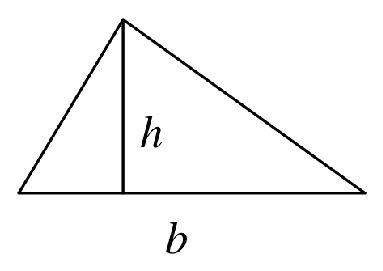
\includegraphics{triangle2.eps}
\end{minipage}

\vspace{1em}

``A área de um triângulo é igual à base vezes a altura sobre dois.''
É dito aos alunos que decorem esta fórmula e então a ``apliquem'' repetidamente nos ``exercícios''.
Foram-se a emoção, a alegria e até mesmo a dor e a frustração do ato criativo.
Não há mais nem um \textsl{problema}.
A pergunta foi feita e respondida ao mesmo tempo -- não restou nada para o aluno fazer.

Permita-me deixar mais claro contra o que estou objetando.
% ficou péssima, a frase original é: Now let me be clear about what I'm objecting to.
Não é sobre fórmulas ou memorizar resultados interessantes.
Isso é legal num contexto e deve ter seu lugar como aprender vocabulário tem -- ajuda você a criar obras de arte mais ricas.
Mas não é o \textsl{fato} de que o triângulo ocupa metade da caixa que importa.
O que importa é a linda \textsl{ideia} de dividi-lo com aquela linha e como isso pode inspirar outras lindas ideias, conduzindo a criativas descobertas em outros problemas -- algo que uma mera apresentação de um resultado nunca pode lhe dar.

Por remover o processo criativo e deixar apenas os resultados deste processo, você praticamente garante que ninguém terá qualquer engajamento real com o assunto.
É como \textsl{dizer} que Michelangelo criou uma linda escultura sem me permitir \textsl{vê-la}.
Como eu seria inspirado por ela?
(E, é claro, na verdade é muito pior que isso -- ao menos eu entendo que \textsl{há} uma arte de escultura que eu estou sendo impedido de apreciar).

% By concentrating on what, and leaving out why... (pagina 5 do original)








% Final do texto:


% commit da pagina 22

Mais importante, a idéia foi do próprio aluno. A classe teve um bom problema para trabalhar, conjecturas foram feitas, as provas foram tentadas e é com isso que o estudante veio. Lógico que levou vários dias e foi o resultado final de uma longa seqüência de fracassos.
Para ser justo, eu fiz a interpretação da prova discretamente. A original era um pouco mais complicada e tinha um monte de verbosidade desnecessária (assim como a ortografia e erros de gramática). Mas eu acho que eu peguei o sentido de por trás disso. E esses defeitos foram todos para o bem, pois eles me deram alguma coisa para fazer, como professor. Eu fui capaz de apontar vários estililos e problemas de lógicas, e o estudante foi então capaz de melhorar a argumentação. Por exemplo, eu não estava completamente satisfeito com uma parte sobre ambas as diagonais sendo diâmetros - eu não acho que foi totalmente óbvio - mas aquilo só queria dizer que havia mais para pensar e mais intendimento para
ser adquirido com a situação. E de fato o aluno foi capaz de preencher essa lacuna muito bem:

\begin{quote}
"Desde que o triângulo tenha girado em torno do meio do círculo, a ponta deve acabar exatamente no oposto de onde começou. É por isso que a diagonal da caixa é um diâmetro."
\end{quote}

Assim, um grande projeto e uma bela parte da matemática. Não tenho a certeza de quem ficou mais orgulhoso, o aluno ou eu. Este é exatamente o tipo de experiência que eu quero que meus alunos tenham.

\vspace{1em}

O problema com o currículo de geometria padrão é que o segredo, experiencia pessoal, de ser um artista esforçando foi praticamente eliminado. A arte da prova foi substituída por um rígido passo-a-passo do padrão sem inspiração de deduções formais. O livro apresenta um conjunto de definições, teoremas e provas, o professor os copia na lousa e os alunos os copiam em seus cadernos. Em seguida, são pedidos para imitá-los nos exercícios. Os que pegar rapidamente o padrão são os "bons" alunos.
O resultado é que o aluno se torna um participante passivo no ato criativo. Os alunos estão
fazendo declarações para encaixar um padrão de prova preexistente, não porque eles o resolvam. Eles estão
sendo treinados para imitar argumentos, não é a intenção deles. Assim, não somente eles não têm idéia do que seus
professores estão dizendo, eles não têm idéia do que eles mesmos estão dizendo.
Mesmo a maneira tradicional em que as definições são apresentadas é uma mentira. Em um esforço para criar uma
ilusão de "clareza" antes de iniciar a cascata típicos de proposições e teoremas, um conjunto
de definições são dadas de forma que as suas declarações e as provas podem ser feitas de forma tão sucinta quanto
possível. Na superfície isso parece bastante inócuo, porque não fazer algumas abreviações para que
coisas possam ser ditas de forma mais econômica? A questão é que as definições importam . Eles vêm de decisões estéticas sobre quais distinções você, como um artista, considera importante. E eles são problemas-criados. Para fazer com que uma definição se destaque e chame a atenção para uma característica ou propriedade estrutural. Historicamente, este sai de foco em um problema, não como um prelúdio para isso. O ponto é que você não começa com definições, você começa com problemas. Ninguém nunca teve um idéia de um número a ser "irracional" até Pitágoras tentar medir a diagonal de um quadrado e descobrir que não poderia ser representado como uma fração. Definições fazem sentido quando um ponto é alcançado em seu argumento que faz a distinção necessária. Fazer definições sem motivação é mais susceptível de causar confusão.
Este é mais um exemplo da maneira que os estudantes são protegido e excluídos do processo matemático. Os estudantes precisam ser capazes de fazer suas próprias definições assim que a necessidade surgir - para formar o próprio debate. Eu não quero alunos dizendo: "a definição, o
teorema, a prova", eu quero vê-los dizendo, "a minha definição, o meu teorema, minha prova". 

% fim do commit da pagina 22

% Commit feito por @alantiel diretamente pelo browser, ver se deu certo ou nao 
% texto da pagina 23


Deixando todas estas reclamações de lado, o verdadeiro problema com este tipo de apresentação é que é tedioso. Eficiência e economia simplesmente não faz boa pedagogia. Eu tenho dificuldade em acreditar que Euclides aprovaria isto, sei que Arquimedes não aprovaria 

SIMPLICIO: Agora espere um minuto. Eu não sei você, mas eu realmente gostava das minhas aulas de geometria no ensino médio. Eu gostava da estrutura e do trabalho feito no rígido formato de prova.

SALVIATI: Eu tenho certeza que você gostava. Você, provavelmente, ainda tem que trabalhar em alguns bons problemas ocasionalmente. Muitas pessoas gostam de aula de geometria (apesar de a maioria odiar). Mas este não é um ponto a favor do atual regime. Ao contrário, o testemunho é poderoso para o fascínio da matemática em si. É difícil arruinar completamente alguma coisa tão bonita, mesmo esta pálida sombra da matemática ainda pode ser atraente e gratificante. Muitas pessoas gostam de pintura-por-números, bem, é uma atividade manual relaxante e colorida. Isso não faz a coisa ser real, no entanto.

SIMPLICIO: Mas eu estou te dizendo, eu gostava. 

SALVIATI: E se você tivesse tido uma experiência mais natural de matemática você teria gostado ainda mais.

Simplício: Então estamos supondo apenas iniciar algumas formas livres para a o ensino da matemática e os alunos irão aprender com que quer que aconteça para aprender? 

SALVIATI: Precisamente. Problemas levarão a outros problemas, a técnica será desenvolvido assim que ela se torne necessária e novos temas surgirão naturalmente. E se isso nunca acontecem em treze anos de escolaridade, quanto interessante ou importante poderia ser? 

SIMPLICIO: Você está completamente louco. 

SALVIATI: Talvez eu seja. Mas, mesmo trabalhando dentro dos moldes convencionais, um bom professor pode orientar a discussão e o fluxo de problemas de forma permitindo que os alunos descobram e inventem a matemática por eles mesmos. O verdadeiro problema é que a burocracia não permite um professor sozinho para fazer isso. Com um currículo definido a seguir, um professor não pode conduzir. Não deve haver padrões e nenhum currículo. Apenas os indivíduos fazendo o que eles acham melhor para seus alunos.

Simplício: Mas então, como as escolas podem garantir que seus alunos terão todos o mesmo conhecimento básico? Como vamos medir com precisão a sua mérito relativo aos outros? 

SALVIATI: Eles não podem e nós não poderemos. Assim como na vida real. Finalmente você tem que encarar o fato de que as pessoas são todas diferentes e isso é bom. De qualquer maneira, não há urgência. Assim, uma pessoa diplomada do ensino médio não conhecer a fórmulas de semi-ângulo  (como se eles conhececem agora!) E dai? Pelo menos essas pessoa viria de com algum tipo de uma idéia do que o assunto é realmente e começaria a ver uma coisa bonita. 


\section*{Conclusão}
Para dar os últimos retoques em minha crítica ao currículo padrão e também como um serviço para a comunidade, apresento agora o primeiro catálogo de cursos para matemática no ensino básico: fundamental e médio (k-12), completamente leal:



% Final do texto comitado pelo browser por @alantiel



\section*{O currículo padrão do ensino de matemática nos EUA}

\begin{description}
\item[MATEMÁTICA NO ENSINO FUNDAMENTAL I.]
A doutrinação começa.
Os alunos aprendem que a matemática não é algo que você faz, mas algo que é feito para você.
A ênfase ainda é ser passivo, preencher tabelas e seguir direções.
As crianças são treinadas para dominar um conjunto complexo de algoritmos para manipular símbolos Hindi, mas sem qualquer vontade real ou curiosidade própria e considerado há apenas alguns séculos atrás como muito difícil para o o adulto médio.
Tabuadas são chatas, assim como os pais, professores e as próprias crianças.

\item[MATEMÁTICA NO ENSINO FUNDAMENTAL II.]
Os alunos são ensinados a ver a matemática como um conjunto de procedimentos, iguais à ritos religiosos, que são eternos e imutáveis.
As tabelas sagradas, ou ``Livros de Matemática'', são entregues e os estudantes aprendam a enfrentar os padres da igreja como ``eles'' (como em ``O que eles querem aqui? Eles querem me dividir?'').
Rebuscados e artificiais ``caça-palavras'' são introduzidos a fim de  fazer o trabalho pesado estúpido da aritmética parecer agradável, por comparação.
Os alunos serão testados em uma ampla gama de termos técnicos desnecessários, tais como ``número inteiro'' e ``propriedades de fração'', sem a menor razão para fazer tais distinções.
Excelente preparação para a Álgebra I. 

\item[ÁLGEBRA I.]
Para não perder tempo precioso pensando em números e seus padrões, este curso foca os símbolos e as regras para a sua manipulação.
A suave discussão narrativa que leva dos antigos problemas da Mesopotâmia à alta arte dos algebristas da Renascença é descartada em favor de algo perturbadoramente quebrado, pós-moderno, sem personagens, enredo ou tema.
A insistência em que todos os números e expressões são colocados em diversas formas causa tanta confusão como o significado de identidade e de igualdade.
Os estudantes também devem por algum motivo memorizar a fórmula quadrática.

\item[GEOMETRIA.]
Isolado do resto do currículo, este curso irá aumentar as esperanças de estudantes que pretendam exercer a atividade matemática, mas significativa e em seguida, destruí-las.
Grosseiras e confusas notações serão introduzidas e sem esforço farão o simples parecer complicado.
O objetivo deste curso é acabar com os últimos vestígios restantes da intuição matemática natural, preparando para a Álgebra II.

\item[ÁLGEBRA II.]
O tema deste curso é o uso inadequado de desmotivado da geometria coordenada.
Seções cônicas são introduzidos em um quadro de coordenadas, de modo a evitar a estética simplicidade de cones e suas seções.
Os alunos vão aprender a reescrever formas quadráticas em muitos formatos sem nenhuma razão aparente.
Funções exponenciais e logarítmicas são, também, introduzidas em Álgebra II, apesar de não serem objetos algébricos, aparentemente simplesmente porque eles tem que ser colocados em algum lugar.
O nome do curso é escolhido para reforçar a ladder mythology.
% Como traduzir "ladder mythology"?
Porque Geometria é ensinada em Álgebra I e sua sequência permanece um mistério.

\item[TRIGONOMETRIA.]
Duas semanas de conteúdo são esticados ao comprimento de um semestre por masturbatórias desculpas.
Fenômenos verdadeiramente interessantes e bonitos, tais como a forma como os lados do um triângulo dependem de seus ângulos, tem a mesma ênfase que irrelevantes abreviaturas e obsoletas convenções de notação, a fim de impedir os estudantes de formar qualquer ideia clara sobre o assunto.
Os alunos aprenderão como dispositivos mnemônicos como ``SohCahToa'' e ``Todos os Estudantes Estudam Cálculo'', em vez de desenvolver um sentimento natural e intuitivo para orientação e simetria.
A medição de triângulos será discutida sem menção da natureza transcendental das funções trigonométricas, ou a linguística e consequentes problemas filosóficos inerentes à tomada de tais medidas.
Calculadoras são necessárias, de modo a ajudar ainda mais estas questões.

\item[PRÉ-CÁLCULO.]
Uma sopa sem sentido de tópicos desconectados.
Principalmente uma tentativa imatura de introduzir métodos analíticos do final do século XIX em ambientes onde eles não são necessários nem úteis.
Definições técnicas de ``limites'' e ``continuidade'' são apresentados a fim de obscurecer a noção intuitivamente evidente de mudança suave.
Como o nome sugere, este curso prepara o estudante para o cálculo, onde a fase final na ofuscação sistemática de quaisquer idéias naturais relacionadas com a forma e o movimento será concluída.

\item[CÁLCULO.]
Este curso irá explorar a matemática do movimento e as melhores formas para enterrá-lo sob uma montanha de formalismo desnecessário.
Apesar de ser uma introdução a ambos os cursos: cálculo diferencial e integral, as idéias simples e profunda de Newton e Leibniz serão descartadas em favor da função mais sofisticada abordagem baseada no desenvolvido como uma resposta a várias crises analítica que realmente não se aplica neste contexto, e que, naturalmente, ser mencionados.
Para ser tomado novamente na faculdade, literalmente. 
\end{description}

\vspace{1em}

\begin{center}
***
\end{center}

\vspace{1em}

E aí está.
A receita completa para desativar permanentemente jovens mentes -- uma cura comprovada por curiosidade.
% Cura comprovada por curiosidade? "proven cure for curiosity"
O que eles fizeram para a matemática!

Há profundidade e beleza de tirar o fôlego comovente nesta forma de arte antiga.
Como é irônico que as pessoas recusam a matemática como a antítese da criatividade\ldots
Eles estão perdendo uma forma de arte mais antiga do que qualquer livro, mais profunda do que qualquer poema e mais abstrata do que qualquer resumo.
E é a escola que fez isso!
Que triste ciclo sem fim de professores inocentes inflingindo danos aos estudantes inocentes.
Nós todos poderíamos estar nos divertindo muito mais.

\begin{description}
\item[SIMPLÍCIO:] Tudo bem, eu estou completamente deprimido. E agora?
\item[SALVIATI:] Bem, eu acho que tenho uma idéia sobre uma pirâmide dentro de um cubo\ldots
\end{description}

\end{document}

